\documentclass[titlepage]{article}
\usepackage{amsmath} \usepackage{amssymb}
\usepackage{fullpage}
\usepackage{graphicx}

\DeclareMathOperator{\arccot}{arccot}

\title{Assignment 7}
\date{\today}
\author{Jerry Jiang\\ TianQi Shi}

\begin{document}
\maketitle

\noindent
\section*{Problem Set 1}
\subsection*{Question 1}

\subsubsection*{1.1}
For part 1.1, I'm going to assume you meant the inverse laplace, instead of the
laplace of the two rational expressions.

I shall prove this using induction, consider the base case: $n = 0$.
We know that $L\{t^0\} = L\{1\} = \frac{1}{s} = \frac{0!}{s^{0 + 1}}$.
So the statement is true for the base case.

Assume that the statement is true for some integer $k \ge 0$. Consider $k + 1$.

Consider the following equation.

$$Y(s) = \frac{(k+1)!}{s^{k+2}}$$

This is equivalent to

$$Y(s) = \frac{k!}{s^{k+1}}\frac{(k+1)}{s}$$

We know from the induction hypothesis that

$$L\{t^k\} = \frac{k!}{s^{k+1}}$$

So therefore

$$Y(s) = L\{t^k\}L\{k+1\}$$

Therefore, by convolution

$$y(t) = \int_{0}^{t}(k+1)(\tau^k) d\tau = t^{k+1}$$

So by the principle of mathematical induction,

$$L\{t^n\} = \frac{n!}{s^{n+1}}$$

\subsubsection*{1.2}
Also, again, assuming that you mean inverse laplace.

$$\frac{1}{(s+2)(s^2 + 1)} + \frac{3}{s^2 + 9}$$

Firstly, we know that

$$L^{-1}\{\frac{3}{s^2 + 9}\} = \sin(3t)$$
$$L^{-1}\{\frac{1}{s+2}\} = e^{-2t}$$
$$L^{-1}\{\frac{1}{s^2 + 1}\} = \sin(t)$$

So,

\begin{align*}
    L^{-1}\{\frac{1}{(s+2)(s^2 + 1)} + \frac{3}{s^2 + 9}\} &=
        \int_{0}^{t} \sin(\tau)e^{-2(t - \tau)} d\tau + \sin(3t)
        \\ &= e^{-2t}\int_{0}^{t} \sin(\tau)e^{2\tau} d\tau + \sin(3t)
\end{align*}

Now we solve the integral.

\begin{align*}
    \int_{0}^{t} \sin(\tau)e^{2\tau} d\tau
    & =\frac{e^{2\tau}}{2}\sin(\tau) \bigg|_0^t - \frac{1}{2}\int_{0}^{t} \cos(\tau)e^{2\tau} d\tau
    \\ &=\frac{e^{2\tau}}{2}\sin(\tau) \bigg|_0^t
    - \frac{1}{2}\bigg(\frac{e^{2\tau}}{2}\cos(\tau) \bigg|_0^t + \frac{1}{2}\int_{0}^{t} \sin(\tau)e^{2\tau} d\tau \bigg)
    \\ &=\frac{e^{2t}}{2}\sin(t)
    - \frac{1}{2}\bigg(\frac{e^{2t}}{2}\cos(t) - \frac{1}{2} + \frac{1}{2}\int_{0}^{t} \sin(\tau)e^{2\tau} d\tau \bigg)
    \\ 2 \int_{0}^{t} \sin(\tau)e^{2\tau} d\tau &= e^{2t}\sin(t)
    - \frac{e^{2t}}{2}\cos(t) + \frac{1}{2} - \frac{1}{2}\int_{0}^{t} \sin(\tau)e^{2\tau} d\tau
    \\ 4\int_{0}^{t} \sin(\tau)e^{2\tau} d\tau &= 2e^{2t}\sin(t)
    - e^{2t}\cos(t) + 1 - \int_{0}^{t} \sin(\tau)e^{2\tau} d\tau
    \\ 5\int_{0}^{t} \sin(\tau)e^{2\tau} d\tau &= 2e^{2t}\sin(t)
    - e^{2t}\cos(t) - 1
    \\ \int_{0}^{t} \sin(\tau)e^{2\tau} d\tau &= \frac{e^{2t}}{5}(2\sin(t) - \cos(t)) - \frac{1}{5}
\end{align*}

So therefore,

\begin{align*}
    L^{-1}\{\frac{1}{(s+2)(s^2 + 1)} + \frac{3}{s^2 + 9}\}
        &= e^{-2t}\int_{0}^{t} \sin(\tau)e^{2\tau} d\tau + \sin(3t)
    \\ &= e^{-2t}\bigg(\frac{e^{2t}}{5}(2\sin(t) - \cos(t)) - \frac{1}{5}\bigg) + \sin(3t)
    \\ &= \frac{1}{5}(2\sin(t) - \cos(t)) - \frac{e^{-2t}}{5} + \sin(3t)
\end{align*}

\subsection*{Question 2}

$$x'' + x' - 6x = 10 - u(t - 4), x(0) = x'(0) = 0$$

First we take the Laplace of both sides
\begin{align*}
    s^2X(s) + sX(s) - 6X(s) &= \frac{10 - e^{-4s}}{s}
    \\ X(s) &= \frac{10 - e^{-4s}}{s(s^2 + s - 6)}
    \\ &= \frac{10 - e^{-4s}}{s(s+3)(s-2)}
\end{align*}

Consider $\frac{1}{s(s+3)(s-2)}$.

\begin{align*}
    L^{-1}\{\frac{1}{s(s+3)(s-2)}\} = L^{-1}\{\frac{1}{s}\} * L^{-1}\{\frac{1}{s+3}\} * L^{-1}\{\frac{1}{s-2}\}
\end{align*}

Consider $L^{-1}\{\frac{1}{s}\} * L^{-1}\{\frac{1}{s+3}\}$.

\begin{align*}
    L^{-1}\{\frac{1}{s}\} * L^{-1}\{\frac{1}{s+3}\} &= \int_0^t e^{-3\tau} d\tau
    \\ &= -\frac{e^{-3t}}{3} + \frac{1}{3}
\end{align*}

We use this value in the second convolution equation.

\begin{align*}
    L^{-1}\{\frac{1}{s}\} * L^{-1}\{\frac{1}{s+3}\} * L^{-1}\{\frac{1}{s-2}\}
    &= \frac{1}{3}\int_0^t (1 - e^{-3\tau})e^{2t - 2\tau} d\tau
    \\ &= \frac{e^{2t}}{3}\int_0^t e^{-2\tau} - e^{-5\tau} d\tau
    \\ &= \frac{e^{2t}}{3} \bigg(-\frac{e^{-2\tau}}{2} + \frac{e^{-5\tau}}{5}\bigg) \bigg|_0^t
    \\ &= \frac{e^{2t}}{3} \bigg(-\frac{e^{-2t}}{2} + \frac{e^{-5t}}{5} + \frac{3}{10}\bigg)
    \\ &= \frac{1}{3} \bigg(-\frac{1}{2} + \frac{e^{-3t}}{5} + \frac{3e^{2t}}{10}\bigg)
\end{align*}

So in total, the final solution is.

$$x(t) = \frac{10}{3}\bigg(-\frac{1}{2} + \frac{e^{-3t}}{5} + \frac{3e^{2t}}{10}\bigg) - \frac{u(t - 4)}{3}\bigg(-\frac{1}{2} + \frac{e^{-3(t - 4)}}{5} + \frac{3e^{2(t - 4)}}{10}\bigg)$$

\section*{Problem Set 2}
\subsection*{Question 1}
\begin{align*}
    L^{-1}\{\frac{1}{s^2(s^2+4)}\} &= L^{-1}\{\frac{1}{s^2}\}L^{-1}\{\frac{1}{s^2+4}\} \\
    &= \int_0^t (t-\tau) \frac{1}{2} \sin(2\tau) d\tau \\
    &= \frac{t}{2} \int_0^t \sin(2\tau) d\tau - \frac{1}{2}\int_0^t \tau \sin(2\tau) d\tau \\
    &= \frac{t}{2}\bigg(\frac{-\cos(2\tau)}{2}\bigg)\bigg|_0^t - \frac{1}{2} \int_0^t \tau \sin(2\tau) d\tau \\
    &= \frac{-t\cos(2t)}{4} + \frac{t}{4} - \frac{1}{2} \int_0^t \tau \sin(2\tau) d\tau
\end{align*}
Using integration by parts,
\begin{align*}
    \int_0^t \tau \sin(2\tau) d\tau &= \tau \bigg(\frac{-\cos(2\tau)}{2}\bigg)\bigg|_0^t - \int_0^t \frac{-\cos(2\tau)}{2} d\tau \\
    &= \frac{-t\cos(2t)}{2} + \frac{1}{2} \int_0^t \cos(2\tau) d\tau \\
    &= \frac{-t\cos(2t)}{2} + \frac{1}{2} \bigg( \sin(\tau)\cos(\tau) \bigg) \bigg|_0^t\\
    &= \frac{-t\cos(2t)}{2} + \frac{\sin(2t)}{4}
\end{align*}
Substituting back,
\begin{align*}
    \frac{-t\cos(2t)}{4} + \frac{t}{4} - \frac{1}{2} \int_0^t \tau \sin(2\tau) d\tau &= \frac{-t\cos(2t)}{4} + \frac{t}{4} - \frac{1}{2} \bigg( \frac{-t\cos(2t)}{2} + \frac{\sin(2t)}{4} \bigg) \\
    &= \frac{-t\cos(2t)}{4} + \frac{t}{4} + \frac{t\cos(2t)}{4} - \frac{\sin(2t)}{8} \\
    &= \frac{t}{4} - \frac{\sin(2t)}{8}
\end{align*}

\subsection*{Question 2}
\begin{align*}
    L^{-1}\{\frac{2s}{(s^2+1)^2}\} &= L^{-1}\{\frac{2}{s^2+1}\}L^{-1}\{\frac{s}{s^2+1}\} \\
    &= \int_0^t 2\sin(t-\tau)\cos(\tau) d\tau \\
    &= 2 \int_0^t \bigg(\sin(t)\cos(\tau) - \cos(t)\sin(\tau)\bigg)\cos(\tau) d\tau \\
    &= 2 \sin(t) \int_0^t \cos^2(\tau) d\tau - 2\cos(t)\int_0^t\sin(\tau)\cos(\tau) d\tau \\
    &= 2 \sin(t) \int_0^t \bigg(\frac{\cos(2\tau)}{2} + \frac{1}{2}\bigg) d\tau - 2\cos(t)\bigg(\frac{\sin^2(t)}{2}\bigg)\bigg|_0^t \\
    &= 2 \sin(t) \bigg( \frac{1}{2}\int_0^t\cos(2\tau)d\tau +  \frac{1}{2}\int_0^t d\tau\bigg) - \sin^2(t)\cos(t) \\
    &= \sin(t) \bigg(\sin(t)\cos(t) + t\bigg) - \sin^2(t)\cos(t) \\
    &= \sin^2(t)\cos(t) + t\sin(t) - \sin^2(t)\cos(t) \\
    &= t\sin(t)
\end{align*}

\section*{Simulation}

First, we found the required state space equations. We have $M\ddot{x}=F$ and $F=-k_px-k_d\dot{x}$ which we can combine into a single second order differential equation, $$M\ddot{x}=-k_px-k_d\dot{x}$$
We define two linear differential equations.
$$y_1(t) = x(t)$$
$$y_2(t) = x'(t)$$
If we differentiate both sides,
$$y_1'(t) = x'(t) = y_2(t)$$
$$y_2'(t) = x''(t) = \frac{-k_py_1(t) - k_dy_2(t)}{M}$$
We substitute these into the state space vector, noting that the constants  are functions of mass $M$. \\
For our first simulation, we decided to set the $k_p$ and $k_d$ values to both $4*220$ (220 because it's the total mass of the system),
because we knew that it would give us two poles at $-2$, which meant that it would be stable.
See the below graph for the simulation results.

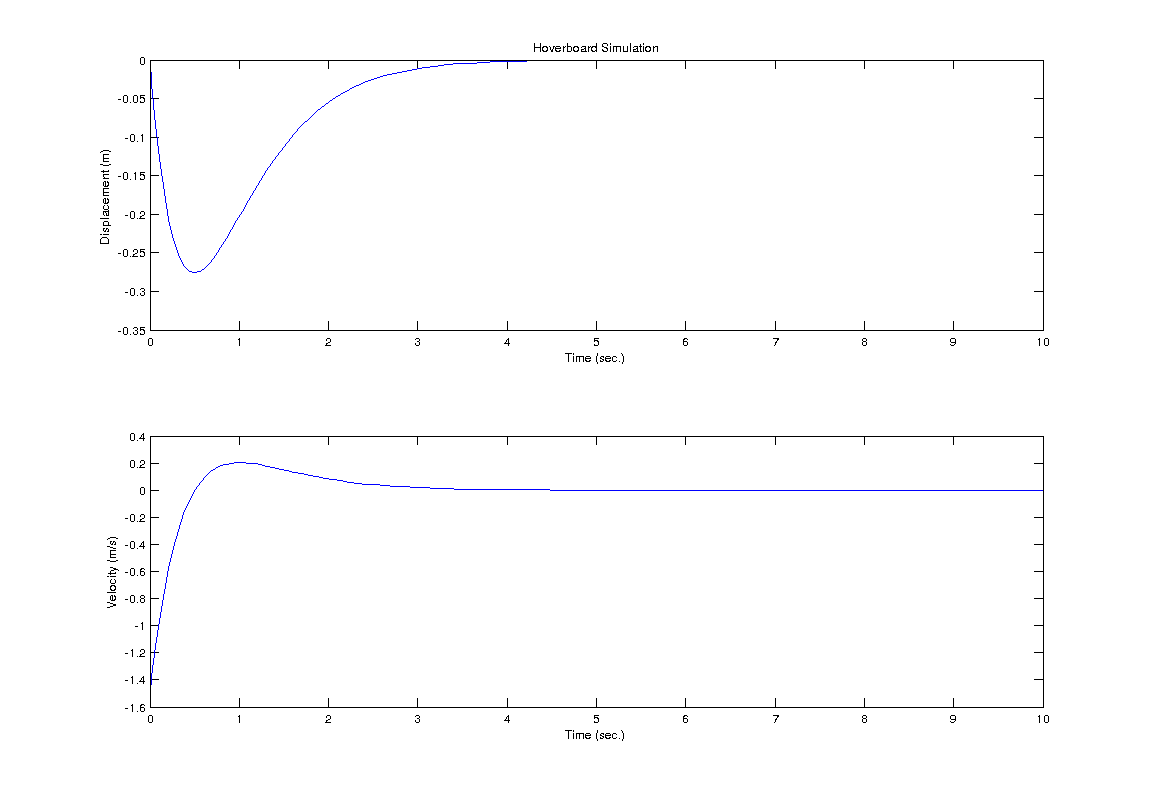
\includegraphics[scale=0.5]{k_pk_d4m.png}

As shown, the displacement does indeed settle back into the original value of 0. As the poles are the same, this also means that the system is critically damped, so there is no oscillation. Instead the hoverboard gradually returns to the resting position smoothly. However, this system results in a trough of approximately -0.275 meters, which is far too low for the requirement of only 0.1 meters. So we decided to increase the $k_p$ and $k_d$ values.

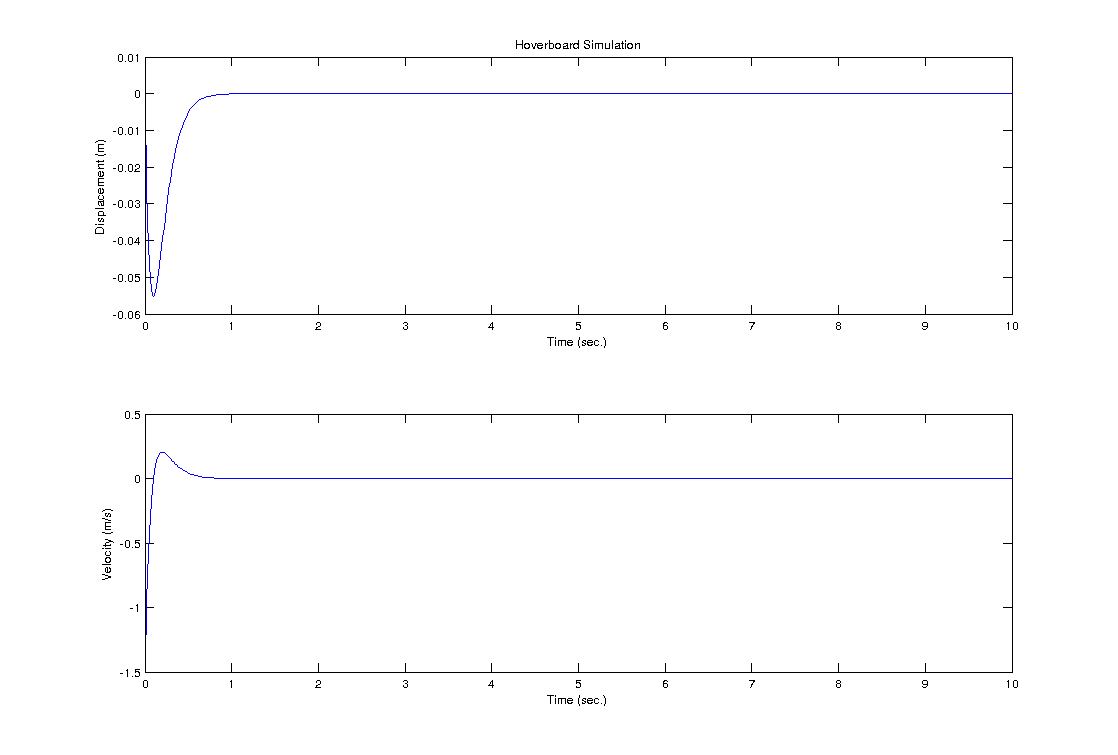
\includegraphics[scale=0.5]{k_p100mk_d20m.png}

At $k_p = 100*220$ and $k_d = 20*220$, we met our goal for a maximum displacement that is less than 0.1 meters. This graph is very similar to the previous simulation, except with the poles at -10 instead of -2. This graph is also critically damped, so there is no oscillation, and it returns to the resting displacement of 0 after reaching a maximum of around -0.055m. We noticed that a much larger $k_p$ and $k_d$ results in a much faster reconciliation.

After satisfying the initial objective, we decided to vary the mass of the person, with our successful $k_p$ and $k_d$. First, we increased the mass to 12000kg combined.

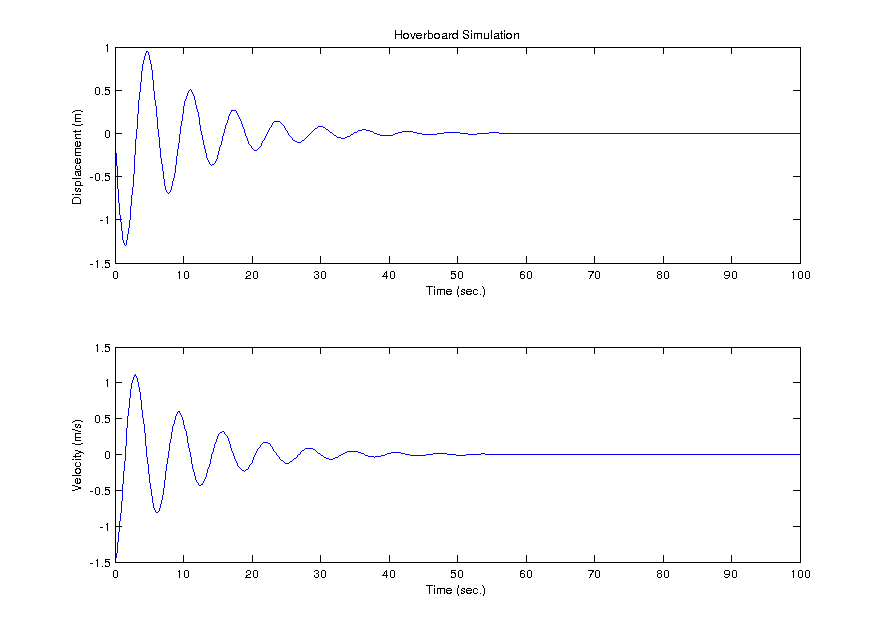
\includegraphics[scale=0.66]{guymass12000k_p100120k_d20120.png}

Firstly, we noticed that the system is still stable, which makes sense since the roots will still have a
negative real part. Secondly, we noticed that the system takes considerably longer to stabilize. This also makes sense, as an increased mass means that we need more power to stabilize in the same amount of time, but we didn't increase the power of the PD controller. Lastly, we noticed
that the system is oscillating as it stabilizes, which also makes sense since the system shouldn't be critically damped anymore. After these observations, we decided to decrease the mass to 12kg combined.

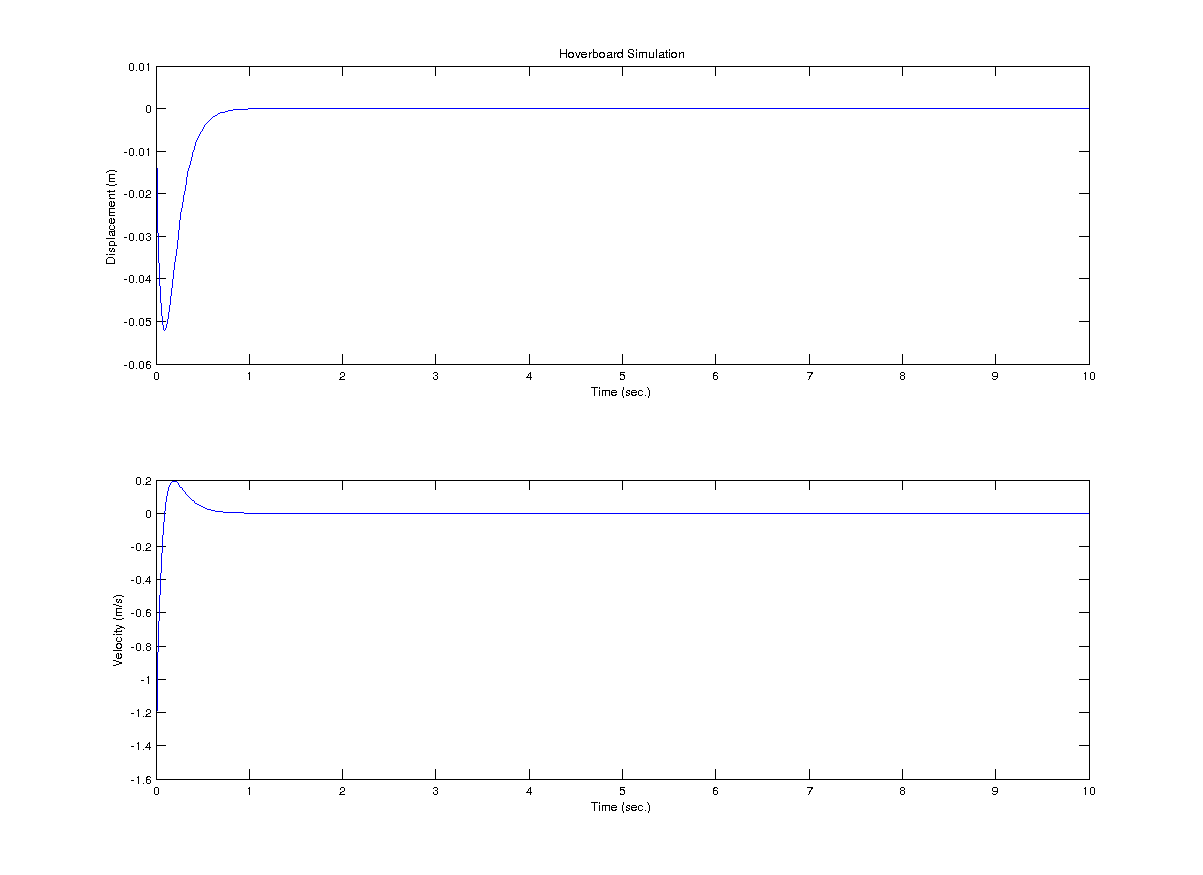
\includegraphics[scale=0.5]{mguy12k_p100120k_d20120.png}

At a mass of 12kg, we noticed that the system is still stable. Additionally, it takes a shorter amount of time for the system to stabilize, and the oscillations appear have disappeared. These all make sense: the poles are still negative, there is less mass for the constant PD controller to counteract, and the system has gone beyond critical damping.

Thus our values of $k_p = 100*220$ and $k_d = 20*220$,  will make the system stable for any weight, but it may not meet the displacement requirement of maximum 10cm drop downward. If we expect very large masses, we must increase $k_p$ and $k_d$ in order to damp at a faster rate. During our state space derivation, we noted that the constants were functions of mass $M$ so there are values of $k_p$ and $k_d$ that would guarantee a displacement requirement for all possible masses. As mass grows, we require the values of $k_p$ and $k_d$ to grow as well.

\end{document}
